% Options for packages loaded elsewhere
\PassOptionsToPackage{unicode}{hyperref}
\PassOptionsToPackage{hyphens}{url}
\PassOptionsToPackage{dvipsnames,svgnames,x11names}{xcolor}
%
\documentclass[
]{article}
\usepackage{amsmath,amssymb}
\usepackage{iftex}
\ifPDFTeX
  \usepackage[T1]{fontenc}
  \usepackage[utf8]{inputenc}
  \usepackage{textcomp} % provide euro and other symbols
\else % if luatex or xetex
  \usepackage{unicode-math} % this also loads fontspec
  \defaultfontfeatures{Scale=MatchLowercase}
  \defaultfontfeatures[\rmfamily]{Ligatures=TeX,Scale=1}
\fi
\usepackage{lmodern}
\ifPDFTeX\else
  % xetex/luatex font selection
\fi
% Use upquote if available, for straight quotes in verbatim environments
\IfFileExists{upquote.sty}{\usepackage{upquote}}{}
\IfFileExists{microtype.sty}{% use microtype if available
  \usepackage[]{microtype}
  \UseMicrotypeSet[protrusion]{basicmath} % disable protrusion for tt fonts
}{}
\makeatletter
\@ifundefined{KOMAClassName}{% if non-KOMA class
  \IfFileExists{parskip.sty}{%
    \usepackage{parskip}
  }{% else
    \setlength{\parindent}{0pt}
    \setlength{\parskip}{6pt plus 2pt minus 1pt}}
}{% if KOMA class
  \KOMAoptions{parskip=half}}
\makeatother
\usepackage{xcolor}
\usepackage[margin=1in]{geometry}
\usepackage{color}
\usepackage{fancyvrb}
\newcommand{\VerbBar}{|}
\newcommand{\VERB}{\Verb[commandchars=\\\{\}]}
\DefineVerbatimEnvironment{Highlighting}{Verbatim}{commandchars=\\\{\}}
% Add ',fontsize=\small' for more characters per line
\usepackage{framed}
\definecolor{shadecolor}{RGB}{248,248,248}
\newenvironment{Shaded}{\begin{snugshade}}{\end{snugshade}}
\newcommand{\AlertTok}[1]{\textcolor[rgb]{0.94,0.16,0.16}{#1}}
\newcommand{\AnnotationTok}[1]{\textcolor[rgb]{0.56,0.35,0.01}{\textbf{\textit{#1}}}}
\newcommand{\AttributeTok}[1]{\textcolor[rgb]{0.13,0.29,0.53}{#1}}
\newcommand{\BaseNTok}[1]{\textcolor[rgb]{0.00,0.00,0.81}{#1}}
\newcommand{\BuiltInTok}[1]{#1}
\newcommand{\CharTok}[1]{\textcolor[rgb]{0.31,0.60,0.02}{#1}}
\newcommand{\CommentTok}[1]{\textcolor[rgb]{0.56,0.35,0.01}{\textit{#1}}}
\newcommand{\CommentVarTok}[1]{\textcolor[rgb]{0.56,0.35,0.01}{\textbf{\textit{#1}}}}
\newcommand{\ConstantTok}[1]{\textcolor[rgb]{0.56,0.35,0.01}{#1}}
\newcommand{\ControlFlowTok}[1]{\textcolor[rgb]{0.13,0.29,0.53}{\textbf{#1}}}
\newcommand{\DataTypeTok}[1]{\textcolor[rgb]{0.13,0.29,0.53}{#1}}
\newcommand{\DecValTok}[1]{\textcolor[rgb]{0.00,0.00,0.81}{#1}}
\newcommand{\DocumentationTok}[1]{\textcolor[rgb]{0.56,0.35,0.01}{\textbf{\textit{#1}}}}
\newcommand{\ErrorTok}[1]{\textcolor[rgb]{0.64,0.00,0.00}{\textbf{#1}}}
\newcommand{\ExtensionTok}[1]{#1}
\newcommand{\FloatTok}[1]{\textcolor[rgb]{0.00,0.00,0.81}{#1}}
\newcommand{\FunctionTok}[1]{\textcolor[rgb]{0.13,0.29,0.53}{\textbf{#1}}}
\newcommand{\ImportTok}[1]{#1}
\newcommand{\InformationTok}[1]{\textcolor[rgb]{0.56,0.35,0.01}{\textbf{\textit{#1}}}}
\newcommand{\KeywordTok}[1]{\textcolor[rgb]{0.13,0.29,0.53}{\textbf{#1}}}
\newcommand{\NormalTok}[1]{#1}
\newcommand{\OperatorTok}[1]{\textcolor[rgb]{0.81,0.36,0.00}{\textbf{#1}}}
\newcommand{\OtherTok}[1]{\textcolor[rgb]{0.56,0.35,0.01}{#1}}
\newcommand{\PreprocessorTok}[1]{\textcolor[rgb]{0.56,0.35,0.01}{\textit{#1}}}
\newcommand{\RegionMarkerTok}[1]{#1}
\newcommand{\SpecialCharTok}[1]{\textcolor[rgb]{0.81,0.36,0.00}{\textbf{#1}}}
\newcommand{\SpecialStringTok}[1]{\textcolor[rgb]{0.31,0.60,0.02}{#1}}
\newcommand{\StringTok}[1]{\textcolor[rgb]{0.31,0.60,0.02}{#1}}
\newcommand{\VariableTok}[1]{\textcolor[rgb]{0.00,0.00,0.00}{#1}}
\newcommand{\VerbatimStringTok}[1]{\textcolor[rgb]{0.31,0.60,0.02}{#1}}
\newcommand{\WarningTok}[1]{\textcolor[rgb]{0.56,0.35,0.01}{\textbf{\textit{#1}}}}
\usepackage{longtable,booktabs,array}
\usepackage{calc} % for calculating minipage widths
% Correct order of tables after \paragraph or \subparagraph
\usepackage{etoolbox}
\makeatletter
\patchcmd\longtable{\par}{\if@noskipsec\mbox{}\fi\par}{}{}
\makeatother
% Allow footnotes in longtable head/foot
\IfFileExists{footnotehyper.sty}{\usepackage{footnotehyper}}{\usepackage{footnote}}
\makesavenoteenv{longtable}
\usepackage{graphicx}
\makeatletter
\def\maxwidth{\ifdim\Gin@nat@width>\linewidth\linewidth\else\Gin@nat@width\fi}
\def\maxheight{\ifdim\Gin@nat@height>\textheight\textheight\else\Gin@nat@height\fi}
\makeatother
% Scale images if necessary, so that they will not overflow the page
% margins by default, and it is still possible to overwrite the defaults
% using explicit options in \includegraphics[width, height, ...]{}
\setkeys{Gin}{width=\maxwidth,height=\maxheight,keepaspectratio}
% Set default figure placement to htbp
\makeatletter
\def\fps@figure{htbp}
\makeatother
\setlength{\emergencystretch}{3em} % prevent overfull lines
\providecommand{\tightlist}{%
  \setlength{\itemsep}{0pt}\setlength{\parskip}{0pt}}
\setcounter{secnumdepth}{5}
\usepackage{fvextra} \DefineVerbatimEnvironment{Highlighting}{Verbatim}{breaklines,commandchars=\\\{\}}
\ifLuaTeX
  \usepackage{selnolig}  % disable illegal ligatures
\fi
\usepackage{bookmark}
\IfFileExists{xurl.sty}{\usepackage{xurl}}{} % add URL line breaks if available
\urlstyle{same}
\hypersetup{
  pdftitle={Other Methods for Dealing with Missingness},
  colorlinks=true,
  linkcolor={Maroon},
  filecolor={Maroon},
  citecolor={Blue},
  urlcolor={blue},
  pdfcreator={LaTeX via pandoc}}

\title{Other Methods for Dealing with Missingness}
\author{}
\date{\vspace{-2.5em}}

\begin{document}
\maketitle

{
\hypersetup{linkcolor=}
\setcounter{tocdepth}{2}
\tableofcontents
}
\section{Introduction}\label{introduction}

We will explore other methods of dealing with missingness, and compare them. We will run each method, and then provide a comparison at the end.

\subsection{Requirements}\label{requirements}

We load the required packages with the code below.

\begin{Shaded}
\begin{Highlighting}[]
\CommentTok{\# List of required packages}
\NormalTok{packages }\OtherTok{\textless{}{-}} \FunctionTok{c}\NormalTok{(}\StringTok{"rpart"}\NormalTok{, }\StringTok{"caret"}\NormalTok{, }\StringTok{"pROC"}\NormalTok{, }\StringTok{"ggplot2"}\NormalTok{, }\StringTok{"dplyr"}\NormalTok{)}

\CommentTok{\# Function to check if a package is installed, and install it if it\textquotesingle{}s missing}
\NormalTok{install\_if\_missing }\OtherTok{\textless{}{-}} \ControlFlowTok{function}\NormalTok{(pkg) \{}
  \ControlFlowTok{if}\NormalTok{ (}\SpecialCharTok{!}\FunctionTok{require}\NormalTok{(pkg, }\AttributeTok{character.only =} \ConstantTok{TRUE}\NormalTok{)) \{}
    \FunctionTok{install.packages}\NormalTok{(pkg, }\AttributeTok{dependencies =} \ConstantTok{TRUE}\NormalTok{)}
\NormalTok{  \}}
\NormalTok{\}}

\CommentTok{\# Install any missing packages}
\FunctionTok{invisible}\NormalTok{(}\FunctionTok{lapply}\NormalTok{(packages, install\_if\_missing))}
\end{Highlighting}
\end{Shaded}

\begin{verbatim}
## Loading required package: rpart
\end{verbatim}

\begin{verbatim}
## Loading required package: caret
\end{verbatim}

\begin{verbatim}
## Loading required package: ggplot2
\end{verbatim}

\begin{verbatim}
## Loading required package: lattice
\end{verbatim}

\begin{verbatim}
## Loading required package: pROC
\end{verbatim}

\begin{verbatim}
## Type 'citation("pROC")' for a citation.
\end{verbatim}

\begin{verbatim}
## 
## Attaching package: 'pROC'
\end{verbatim}

\begin{verbatim}
## The following objects are masked from 'package:stats':
## 
##     cov, smooth, var
\end{verbatim}

\begin{verbatim}
## Loading required package: dplyr
\end{verbatim}

\begin{verbatim}
## 
## Attaching package: 'dplyr'
\end{verbatim}

\begin{verbatim}
## The following objects are masked from 'package:stats':
## 
##     filter, lag
\end{verbatim}

\begin{verbatim}
## The following objects are masked from 'package:base':
## 
##     intersect, setdiff, setequal, union
\end{verbatim}

\begin{Shaded}
\begin{Highlighting}[]
\CommentTok{\# Load the necessary packages}
\FunctionTok{lapply}\NormalTok{(packages, library, }\AttributeTok{character.only =} \ConstantTok{TRUE}\NormalTok{)}
\end{Highlighting}
\end{Shaded}

\begin{verbatim}
## [[1]]
##  [1] "dplyr"     "pROC"      "caret"     "lattice"   "ggplot2"   "rpart"    
##  [7] "stats"     "graphics"  "grDevices" "utils"     "datasets"  "methods"  
## [13] "base"     
## 
## [[2]]
##  [1] "dplyr"     "pROC"      "caret"     "lattice"   "ggplot2"   "rpart"    
##  [7] "stats"     "graphics"  "grDevices" "utils"     "datasets"  "methods"  
## [13] "base"     
## 
## [[3]]
##  [1] "dplyr"     "pROC"      "caret"     "lattice"   "ggplot2"   "rpart"    
##  [7] "stats"     "graphics"  "grDevices" "utils"     "datasets"  "methods"  
## [13] "base"     
## 
## [[4]]
##  [1] "dplyr"     "pROC"      "caret"     "lattice"   "ggplot2"   "rpart"    
##  [7] "stats"     "graphics"  "grDevices" "utils"     "datasets"  "methods"  
## [13] "base"     
## 
## [[5]]
##  [1] "dplyr"     "pROC"      "caret"     "lattice"   "ggplot2"   "rpart"    
##  [7] "stats"     "graphics"  "grDevices" "utils"     "datasets"  "methods"  
## [13] "base"
\end{verbatim}

\begin{Shaded}
\begin{Highlighting}[]
\CommentTok{\# rpart      {-} Recursive partitioning for decision trees}
\CommentTok{\# caret      {-} For confusion matrix and precision/recall calculations}
\CommentTok{\# pROC       {-} For ROC curve}
\CommentTok{\# ggplot2    {-} For plotting}
\CommentTok{\# dplyr      {-} For data manipulation}
\end{Highlighting}
\end{Shaded}

\section{Other Methods to Deal with Missingness}\label{other-methods-to-deal-with-missingness}

\subsection{\texorpdfstring{Analysis with Missingness Encoded as \texttt{?}}{Analysis with Missingness Encoded as ?}}\label{analysis-with-missingness-encoded-as}

This treats missingness as its own category.

\begin{Shaded}
\begin{Highlighting}[]
\CommentTok{\# Get the current working directory}
\NormalTok{current\_dir }\OtherTok{\textless{}{-}} \FunctionTok{getwd}\NormalTok{()}
\FunctionTok{cat}\NormalTok{(}\StringTok{"Current directory:"}\NormalTok{, current\_dir, }\StringTok{"}\SpecialCharTok{\textbackslash{}n}\StringTok{"}\NormalTok{)}
\end{Highlighting}
\end{Shaded}

\begin{verbatim}
## Current directory: C:/Users/megar/Documents/Code/Data Science Toolbox/dst-group-project-1/VivekP
\end{verbatim}

\begin{Shaded}
\begin{Highlighting}[]
\CommentTok{\# Get the parent directory}
\NormalTok{parent\_dir }\OtherTok{\textless{}{-}} \FunctionTok{dirname}\NormalTok{(current\_dir)}
\FunctionTok{cat}\NormalTok{(}\StringTok{"Parent directory:"}\NormalTok{, parent\_dir, }\StringTok{"}\SpecialCharTok{\textbackslash{}n}\StringTok{"}\NormalTok{)}
\end{Highlighting}
\end{Shaded}

\begin{verbatim}
## Parent directory: C:/Users/megar/Documents/Code/Data Science Toolbox/dst-group-project-1
\end{verbatim}

\begin{Shaded}
\begin{Highlighting}[]
\CommentTok{\# Set the working directory to the parent directory}
\FunctionTok{setwd}\NormalTok{(parent\_dir)}
\FunctionTok{cat}\NormalTok{(}\StringTok{"New working directory:"}\NormalTok{, }\FunctionTok{getwd}\NormalTok{(), }\StringTok{"}\SpecialCharTok{\textbackslash{}n}\StringTok{"}\NormalTok{)}
\end{Highlighting}
\end{Shaded}

\begin{verbatim}
## New working directory: C:/Users/megar/Documents/Code/Data Science Toolbox/dst-group-project-1
\end{verbatim}

\begin{Shaded}
\begin{Highlighting}[]
\CommentTok{\# Load the training and test datasets}
\NormalTok{X\_train }\OtherTok{\textless{}{-}} \FunctionTok{read.csv}\NormalTok{(}\StringTok{"data/X\_train\_smote.csv"}\NormalTok{, }\AttributeTok{row.names =} \DecValTok{1}\NormalTok{)  }\CommentTok{\# Load the SMOTE transformed training features}
\NormalTok{y\_train }\OtherTok{\textless{}{-}} \FunctionTok{read.csv}\NormalTok{(}\StringTok{"data/y\_train\_smote.csv"}\NormalTok{, }\AttributeTok{row.names =} \DecValTok{1}\NormalTok{)  }\CommentTok{\# Load the SMOTE transformed training labels}
\NormalTok{X\_test }\OtherTok{\textless{}{-}} \FunctionTok{read.csv}\NormalTok{(}\StringTok{"data/X\_test.csv"}\NormalTok{, }\AttributeTok{row.names =} \DecValTok{1}\NormalTok{)    }\CommentTok{\# Load the test features}
\NormalTok{y\_test }\OtherTok{\textless{}{-}} \FunctionTok{read.csv}\NormalTok{(}\StringTok{"data/y\_test.csv"}\NormalTok{, }\AttributeTok{row.names =} \DecValTok{1}\NormalTok{)    }\CommentTok{\# Load the test labels}

\CommentTok{\# Combine X\_train and y\_train into one data frame for rpart}
\NormalTok{train\_data }\OtherTok{\textless{}{-}} \FunctionTok{cbind}\NormalTok{(X\_train, y\_train)}

\CommentTok{\# Drop the "education" column from the training data if it exists}
\NormalTok{train\_data }\OtherTok{\textless{}{-}}\NormalTok{ train\_data[, }\SpecialCharTok{!}\FunctionTok{names}\NormalTok{(train\_data) }\SpecialCharTok{\%in\%} \StringTok{"education"}\NormalTok{]}

\CommentTok{\# Replace NAs with "?" for both training and test datasets}
\NormalTok{train\_data[}\FunctionTok{is.na}\NormalTok{(train\_data)] }\OtherTok{\textless{}{-}} \StringTok{"?"}
\NormalTok{X\_test[}\FunctionTok{is.na}\NormalTok{(X\_test)] }\OtherTok{\textless{}{-}} \StringTok{"?"}

\CommentTok{\# Fit the classification tree using rpart}
\NormalTok{fit }\OtherTok{\textless{}{-}} \FunctionTok{rpart}\NormalTok{(income }\SpecialCharTok{\textasciitilde{}}\NormalTok{ ., }\AttributeTok{data =}\NormalTok{ train\_data, }\AttributeTok{method =} \StringTok{"class"}\NormalTok{, }\AttributeTok{control =} \FunctionTok{rpart.control}\NormalTok{(}\AttributeTok{cp =} \FloatTok{1e{-}6}\NormalTok{))}

\CommentTok{\# Get the cost{-}complexity pruning table and identify the best cp based on minimum xerror}
\NormalTok{cptable }\OtherTok{\textless{}{-}}\NormalTok{ fit}\SpecialCharTok{$}\NormalTok{cptable}
\NormalTok{best\_cp }\OtherTok{\textless{}{-}}\NormalTok{ cptable[}\FunctionTok{which.min}\NormalTok{(cptable[,}\StringTok{"xerror"}\NormalTok{]), }\StringTok{"CP"}\NormalTok{]}
\FunctionTok{cat}\NormalTok{(}\StringTok{"Best CP:"}\NormalTok{, best\_cp, }\StringTok{"}\SpecialCharTok{\textbackslash{}n}\StringTok{"}\NormalTok{)}
\end{Highlighting}
\end{Shaded}

\begin{verbatim}
## Best CP: 9.903278e-05
\end{verbatim}

\begin{Shaded}
\begin{Highlighting}[]
\CommentTok{\# Prune the tree using the best cp}
\NormalTok{pruned\_tree }\OtherTok{\textless{}{-}} \FunctionTok{prune}\NormalTok{(fit, }\AttributeTok{cp =}\NormalTok{ best\_cp)}

\CommentTok{\# Get predicted probabilities for the positive class}
\NormalTok{pred\_probs }\OtherTok{\textless{}{-}} \FunctionTok{predict}\NormalTok{(pruned\_tree, X\_test, }\AttributeTok{type =} \StringTok{"prob"}\NormalTok{)[, }\StringTok{"\textless{}=50K"}\NormalTok{]  }\CommentTok{\# Adjust based on your positive class}

\CommentTok{\# Compute ROC curve for the model with predictions}
\NormalTok{roc\_curve\_model\_encoded }\OtherTok{\textless{}{-}} \FunctionTok{roc}\NormalTok{(y\_test[, }\DecValTok{1}\NormalTok{], pred\_probs, }\AttributeTok{levels =} \FunctionTok{c}\NormalTok{(}\StringTok{"\textless{}=50K"}\NormalTok{, }\StringTok{"\textgreater{}50K"}\NormalTok{))}
\end{Highlighting}
\end{Shaded}

\begin{verbatim}
## Setting direction: controls > cases
\end{verbatim}

\begin{Shaded}
\begin{Highlighting}[]
\CommentTok{\# Calculate AUC for the model}
\NormalTok{auc\_value\_model\_encoded }\OtherTok{\textless{}{-}} \FunctionTok{auc}\NormalTok{(roc\_curve\_model\_encoded)}

\CommentTok{\# Print AUC value for the model}
\FunctionTok{cat}\NormalTok{(}\StringTok{"AUC for Model (Missing Data Encoded):"}\NormalTok{, auc\_value\_model\_encoded, }\StringTok{"}\SpecialCharTok{\textbackslash{}n}\StringTok{"}\NormalTok{)}
\end{Highlighting}
\end{Shaded}

\begin{verbatim}
## AUC for Model (Missing Data Encoded): 0.8885526
\end{verbatim}

\begin{Shaded}
\begin{Highlighting}[]
\CommentTok{\# Create a data frame for the model\textquotesingle{}s ROC data}
\NormalTok{roc\_data\_model\_encoded }\OtherTok{\textless{}{-}} \FunctionTok{data.frame}\NormalTok{(}
  \AttributeTok{FPR =} \DecValTok{1} \SpecialCharTok{{-}}\NormalTok{ roc\_curve\_model\_encoded}\SpecialCharTok{$}\NormalTok{specificities,  }\CommentTok{\# False Positive Rate}
  \AttributeTok{TPR =}\NormalTok{ roc\_curve\_model\_encoded}\SpecialCharTok{$}\NormalTok{sensitivities         }\CommentTok{\# True Positive Rate}
\NormalTok{)}
\end{Highlighting}
\end{Shaded}

\subsection{Complete Case Analysis}\label{complete-case-analysis}

We start with a simple method of dealing with missing data: simply deleting all missing data. This is not really a good strategy here because we have about 50000 observations and 3000 missing some values. This was not considered a negligible amount of missingness, but we will just consider this as a baseline.

\begin{Shaded}
\begin{Highlighting}[]
\CommentTok{\# Remove rows with missing data from the training and test sets}
\NormalTok{train\_data[train\_data }\SpecialCharTok{==} \StringTok{"?"}\NormalTok{] }\OtherTok{\textless{}{-}} \ConstantTok{NA}
\NormalTok{train\_data }\OtherTok{\textless{}{-}} \FunctionTok{na.omit}\NormalTok{(train\_data)}

\CommentTok{\# Fit the classification tree using rpart}
\NormalTok{fit }\OtherTok{\textless{}{-}} \FunctionTok{rpart}\NormalTok{(income }\SpecialCharTok{\textasciitilde{}}\NormalTok{ ., }\AttributeTok{data =}\NormalTok{ train\_data, }\AttributeTok{method =} \StringTok{"class"}\NormalTok{, }\AttributeTok{control =} \FunctionTok{rpart.control}\NormalTok{(}\AttributeTok{cp =} \FloatTok{1e{-}6}\NormalTok{))}

\CommentTok{\# Get the cost{-}complexity pruning table and identify the best cp based on minimum xerror}
\NormalTok{cptable }\OtherTok{\textless{}{-}}\NormalTok{ fit}\SpecialCharTok{$}\NormalTok{cptable}
\NormalTok{best\_cp }\OtherTok{\textless{}{-}}\NormalTok{ cptable[}\FunctionTok{which.min}\NormalTok{(cptable[,}\StringTok{"xerror"}\NormalTok{]), }\StringTok{"CP"}\NormalTok{]}
\FunctionTok{cat}\NormalTok{(}\StringTok{"Best CP:"}\NormalTok{, best\_cp, }\StringTok{"}\SpecialCharTok{\textbackslash{}n}\StringTok{"}\NormalTok{)}
\end{Highlighting}
\end{Shaded}

\begin{verbatim}
## Best CP: 9.078005e-05
\end{verbatim}

\begin{Shaded}
\begin{Highlighting}[]
\CommentTok{\# Prune the tree using the best cp}
\NormalTok{pruned\_tree }\OtherTok{\textless{}{-}} \FunctionTok{prune}\NormalTok{(fit, }\AttributeTok{cp =}\NormalTok{ best\_cp)}

\CommentTok{\# Get predicted probabilities for the positive class}
\NormalTok{pred\_probs }\OtherTok{\textless{}{-}} \FunctionTok{predict}\NormalTok{(pruned\_tree, X\_test, }\AttributeTok{type =} \StringTok{"prob"}\NormalTok{)[, }\StringTok{"\textless{}=50K"}\NormalTok{]  }\CommentTok{\# Adjust based on your positive class}

\CommentTok{\# Compute ROC curve for the model with predictions}
\NormalTok{roc\_curve\_model\_deleted }\OtherTok{\textless{}{-}} \FunctionTok{roc}\NormalTok{(y\_test[, }\DecValTok{1}\NormalTok{], pred\_probs, }\AttributeTok{levels =} \FunctionTok{c}\NormalTok{(}\StringTok{"\textless{}=50K"}\NormalTok{, }\StringTok{"\textgreater{}50K"}\NormalTok{))}
\end{Highlighting}
\end{Shaded}

\begin{verbatim}
## Setting direction: controls > cases
\end{verbatim}

\begin{Shaded}
\begin{Highlighting}[]
\CommentTok{\# Calculate AUC for the model}
\NormalTok{auc\_value\_model\_deleted }\OtherTok{\textless{}{-}} \FunctionTok{auc}\NormalTok{(roc\_curve\_model\_deleted)}

\CommentTok{\# Print AUC value for the model}
\FunctionTok{cat}\NormalTok{(}\StringTok{"AUC for Model (Missing Data Deleted):"}\NormalTok{, auc\_value\_model\_deleted, }\StringTok{"}\SpecialCharTok{\textbackslash{}n}\StringTok{"}\NormalTok{)}
\end{Highlighting}
\end{Shaded}

\begin{verbatim}
## AUC for Model (Missing Data Deleted): 0.8887446
\end{verbatim}

\begin{Shaded}
\begin{Highlighting}[]
\CommentTok{\# Create a data frame for the model\textquotesingle{}s ROC data}
\NormalTok{roc\_data\_model\_deleted }\OtherTok{\textless{}{-}} \FunctionTok{data.frame}\NormalTok{(}
  \AttributeTok{FPR =} \DecValTok{1} \SpecialCharTok{{-}}\NormalTok{ roc\_curve\_model\_deleted}\SpecialCharTok{$}\NormalTok{specificities,  }\CommentTok{\# False Positive Rate}
  \AttributeTok{TPR =}\NormalTok{ roc\_curve\_model\_deleted}\SpecialCharTok{$}\NormalTok{sensitivities         }\CommentTok{\# True Positive Rate}
\NormalTok{)}
\end{Highlighting}
\end{Shaded}

\subsection{Surrogate Splits}\label{surrogate-splits}

We reuse the code from the previous file.

\textbf{NOTE}: We preferred to do this rather than saving the files and loading them as it sometimes led to non-reproducible issues for the other group members.

\begin{Shaded}
\begin{Highlighting}[]
\CommentTok{\# NEED TO RELOAD DATA: We deleted some of it before. We preferred to do it this way rather than changing the order}
\CommentTok{\# of the methods to avoid reloading it. This is because we wanted the simplest methods first.}

\CommentTok{\# Get the current working directory}
\NormalTok{current\_dir }\OtherTok{\textless{}{-}} \FunctionTok{getwd}\NormalTok{()}
\FunctionTok{cat}\NormalTok{(}\StringTok{"Current directory:"}\NormalTok{, current\_dir, }\StringTok{"}\SpecialCharTok{\textbackslash{}n}\StringTok{"}\NormalTok{)}
\end{Highlighting}
\end{Shaded}

\begin{verbatim}
## Current directory: C:/Users/megar/Documents/Code/Data Science Toolbox/dst-group-project-1/VivekP
\end{verbatim}

\begin{Shaded}
\begin{Highlighting}[]
\CommentTok{\# Get the parent directory}
\NormalTok{parent\_dir }\OtherTok{\textless{}{-}} \FunctionTok{dirname}\NormalTok{(current\_dir)}
\FunctionTok{cat}\NormalTok{(}\StringTok{"Parent directory:"}\NormalTok{, parent\_dir, }\StringTok{"}\SpecialCharTok{\textbackslash{}n}\StringTok{"}\NormalTok{)}
\end{Highlighting}
\end{Shaded}

\begin{verbatim}
## Parent directory: C:/Users/megar/Documents/Code/Data Science Toolbox/dst-group-project-1
\end{verbatim}

\begin{Shaded}
\begin{Highlighting}[]
\CommentTok{\# Set the working directory to the parent directory}
\FunctionTok{setwd}\NormalTok{(parent\_dir)}
\FunctionTok{cat}\NormalTok{(}\StringTok{"New working directory:"}\NormalTok{, }\FunctionTok{getwd}\NormalTok{(), }\StringTok{"}\SpecialCharTok{\textbackslash{}n}\StringTok{"}\NormalTok{)}
\end{Highlighting}
\end{Shaded}

\begin{verbatim}
## New working directory: C:/Users/megar/Documents/Code/Data Science Toolbox/dst-group-project-1
\end{verbatim}

\begin{Shaded}
\begin{Highlighting}[]
\CommentTok{\# Load the training and test datasets}
\NormalTok{X\_train }\OtherTok{\textless{}{-}} \FunctionTok{read.csv}\NormalTok{(}\StringTok{"data/X\_train\_smote.csv"}\NormalTok{, }\AttributeTok{row.names =} \DecValTok{1}\NormalTok{)  }\CommentTok{\# Load the SMOTE transformed training features}
\NormalTok{y\_train }\OtherTok{\textless{}{-}} \FunctionTok{read.csv}\NormalTok{(}\StringTok{"data/y\_train\_smote.csv"}\NormalTok{, }\AttributeTok{row.names =} \DecValTok{1}\NormalTok{)  }\CommentTok{\# Load the SMOTE transformed training labels}
\NormalTok{X\_test }\OtherTok{\textless{}{-}} \FunctionTok{read.csv}\NormalTok{(}\StringTok{"data/X\_test.csv"}\NormalTok{, }\AttributeTok{row.names =} \DecValTok{1}\NormalTok{)    }\CommentTok{\# Load the test features}
\NormalTok{y\_test }\OtherTok{\textless{}{-}} \FunctionTok{read.csv}\NormalTok{(}\StringTok{"data/y\_test.csv"}\NormalTok{, }\AttributeTok{row.names =} \DecValTok{1}\NormalTok{)    }\CommentTok{\# Load the test labels}

\CommentTok{\# Combine X\_train and y\_train into one data frame for rpart}
\NormalTok{train\_data }\OtherTok{\textless{}{-}} \FunctionTok{cbind}\NormalTok{(X\_train, y\_train)}

\CommentTok{\# Drop the "education" column from the training data if it exists}
\NormalTok{train\_data }\OtherTok{\textless{}{-}}\NormalTok{ train\_data[, }\SpecialCharTok{!}\FunctionTok{names}\NormalTok{(train\_data) }\SpecialCharTok{\%in\%} \StringTok{"education"}\NormalTok{]}

\CommentTok{\# Fit the classification tree using rpart}
\NormalTok{fit }\OtherTok{\textless{}{-}} \FunctionTok{rpart}\NormalTok{(income }\SpecialCharTok{\textasciitilde{}}\NormalTok{ ., }\AttributeTok{data =}\NormalTok{ train\_data, }\AttributeTok{method =} \StringTok{"class"}\NormalTok{, }\AttributeTok{control =} \FunctionTok{rpart.control}\NormalTok{(}\AttributeTok{cp =} \FloatTok{1e{-}6}\NormalTok{))}

\CommentTok{\# Get the cost{-}complexity pruning table and identify the best cp based on minimum xerror}
\NormalTok{cptable }\OtherTok{\textless{}{-}}\NormalTok{ fit}\SpecialCharTok{$}\NormalTok{cptable}
\NormalTok{best\_cp }\OtherTok{\textless{}{-}}\NormalTok{ cptable[}\FunctionTok{which.min}\NormalTok{(cptable[,}\StringTok{"xerror"}\NormalTok{]), }\StringTok{"CP"}\NormalTok{]}
\FunctionTok{cat}\NormalTok{(}\StringTok{"Best CP:"}\NormalTok{, best\_cp, }\StringTok{"}\SpecialCharTok{\textbackslash{}n}\StringTok{"}\NormalTok{)}
\end{Highlighting}
\end{Shaded}

\begin{verbatim}
## Best CP: 9.903278e-05
\end{verbatim}

\begin{Shaded}
\begin{Highlighting}[]
\CommentTok{\# Prune the tree using the best cp}
\NormalTok{pruned\_tree }\OtherTok{\textless{}{-}} \FunctionTok{prune}\NormalTok{(fit, }\AttributeTok{cp =}\NormalTok{ best\_cp)}

\CommentTok{\# Get predicted probabilities for the positive class}
\NormalTok{pred\_probs }\OtherTok{\textless{}{-}} \FunctionTok{predict}\NormalTok{(pruned\_tree, X\_test, }\AttributeTok{type =} \StringTok{"prob"}\NormalTok{)[, }\StringTok{"\textless{}=50K"}\NormalTok{]  }\CommentTok{\# Adjust based on your positive class}

\CommentTok{\# Compute ROC curve for the model with predictions}
\NormalTok{roc\_curve\_model }\OtherTok{\textless{}{-}} \FunctionTok{roc}\NormalTok{(y\_test[, }\DecValTok{1}\NormalTok{], pred\_probs, }\AttributeTok{levels =} \FunctionTok{c}\NormalTok{(}\StringTok{"\textless{}=50K"}\NormalTok{, }\StringTok{"\textgreater{}50K"}\NormalTok{))}
\end{Highlighting}
\end{Shaded}

\begin{verbatim}
## Setting direction: controls > cases
\end{verbatim}

\begin{Shaded}
\begin{Highlighting}[]
\CommentTok{\# Calculate AUC for the model}
\NormalTok{auc\_value\_model }\OtherTok{\textless{}{-}} \FunctionTok{auc}\NormalTok{(roc\_curve\_model)}

\CommentTok{\# Print AUC value for the model}
\FunctionTok{cat}\NormalTok{(}\StringTok{"AUC for Model:"}\NormalTok{, auc\_value\_model, }\StringTok{"}\SpecialCharTok{\textbackslash{}n}\StringTok{"}\NormalTok{)}
\end{Highlighting}
\end{Shaded}

\begin{verbatim}
## AUC for Model: 0.8885526
\end{verbatim}

\begin{Shaded}
\begin{Highlighting}[]
\CommentTok{\# Create a data frame for the model\textquotesingle{}s ROC data}
\NormalTok{roc\_data\_model }\OtherTok{\textless{}{-}} \FunctionTok{data.frame}\NormalTok{(}
  \AttributeTok{FPR =} \DecValTok{1} \SpecialCharTok{{-}}\NormalTok{ roc\_curve\_model}\SpecialCharTok{$}\NormalTok{specificities,  }\CommentTok{\# False Positive Rate}
  \AttributeTok{TPR =}\NormalTok{ roc\_curve\_model}\SpecialCharTok{$}\NormalTok{sensitivities         }\CommentTok{\# True Positive Rate}
\NormalTok{)}
\end{Highlighting}
\end{Shaded}

\section{Comparisons of Performance}\label{comparisons-of-performance}

We compare the ROC curves obtained from each method.

\begin{Shaded}
\begin{Highlighting}[]
\CommentTok{\# Create the plot for the saved ROC curve}
\FunctionTok{plot}\NormalTok{(roc\_data\_model}\SpecialCharTok{$}\NormalTok{FPR, roc\_data\_model}\SpecialCharTok{$}\NormalTok{TPR, }\AttributeTok{type =} \StringTok{"l"}\NormalTok{, }\AttributeTok{col =} \StringTok{"red"}\NormalTok{, }\AttributeTok{lwd =} \DecValTok{2}\NormalTok{, }
     \AttributeTok{xlim =} \FunctionTok{c}\NormalTok{(}\DecValTok{0}\NormalTok{, }\DecValTok{1}\NormalTok{), }\AttributeTok{ylim =} \FunctionTok{c}\NormalTok{(}\DecValTok{0}\NormalTok{, }\DecValTok{1}\NormalTok{), }
     \AttributeTok{main =} \StringTok{"ROC Curves Comparison"}\NormalTok{, }
     \AttributeTok{xlab =} \StringTok{"False Positive Rate"}\NormalTok{, }
     \AttributeTok{ylab =} \StringTok{"True Positive Rate"}\NormalTok{)}

\CommentTok{\# Add the ROC curve for the model with missing data deleted}
\FunctionTok{lines}\NormalTok{(roc\_data\_model\_deleted}\SpecialCharTok{$}\NormalTok{FPR, roc\_data\_model\_deleted}\SpecialCharTok{$}\NormalTok{TPR, }\AttributeTok{col =} \StringTok{"blue"}\NormalTok{, }\AttributeTok{lwd =} \DecValTok{2}\NormalTok{)}

\CommentTok{\# Add the ROC curve for the model with missing data encoded as "?"}
\FunctionTok{lines}\NormalTok{(roc\_data\_model\_encoded}\SpecialCharTok{$}\NormalTok{FPR, roc\_data\_model\_encoded}\SpecialCharTok{$}\NormalTok{TPR, }\AttributeTok{col =} \StringTok{"green"}\NormalTok{, }\AttributeTok{lwd =} \DecValTok{2}\NormalTok{)}

\CommentTok{\# Add a diagonal line for random guessing}
\FunctionTok{abline}\NormalTok{(}\DecValTok{0}\NormalTok{, }\DecValTok{1}\NormalTok{, }\AttributeTok{lty =} \DecValTok{2}\NormalTok{, }\AttributeTok{col =} \StringTok{"grey"}\NormalTok{)}

\CommentTok{\# Add a legend to the plot}
\FunctionTok{legend}\NormalTok{(}\StringTok{"bottomright"}\NormalTok{, }\AttributeTok{legend =} \FunctionTok{c}\NormalTok{(}\StringTok{"ROC Curve (Surrogate Splits)"}\NormalTok{, }\StringTok{"ROC Curve (Missing Data Deleted)"}\NormalTok{, }\StringTok{"ROC Curve (Missing Data Encoded)"}\NormalTok{),}
       \AttributeTok{col =} \FunctionTok{c}\NormalTok{(}\StringTok{"red"}\NormalTok{, }\StringTok{"blue"}\NormalTok{, }\StringTok{"green"}\NormalTok{), }\AttributeTok{lwd =} \DecValTok{2}\NormalTok{)}
\end{Highlighting}
\end{Shaded}

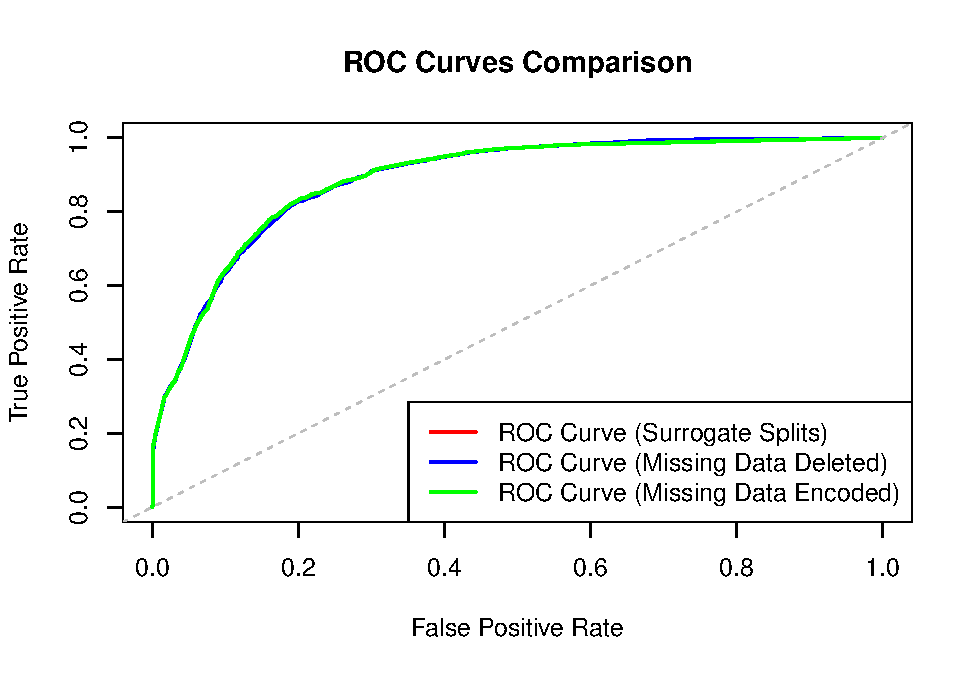
\includegraphics{04-02.3-MissingnessMethodsWithSmote_files/figure-latex/unnamed-chunk-4-1.pdf}

The results shocked us. The tree was quite robust to the method we chose, and the ROC curves and AUC were almost identical.

Having exhausted most of the methods of dealing with missingness we explored, as well as the use of SMOTE to treat imbalance, we moved to considering ensembles.

\end{document}
